\chapter{\poy Quick Start}

\section{Requirements: software and hardware}

\subsection{Software}
\poy is a platform-independent, open-source program that can be compiled for many operating systems and hardware configurations, including Mac OSX, Microsoft Windows XP, and Linux. %\poy \emph{binaries}\index{general}{binaries} (compiled application file) is the only piece of software necessary to run \poy%. 
The intuitive graphical user interface of \poy provides all the functionality for running analyses using pull-down menus and field selections, as well as creating and running \poy scripts. Some utility programs (such as Notepad and Ghostscript for Windows, TextEdit for Mac, or Nano for Linux), can help preparing \poy scripts and formatting data files, while others (such as Adobe Acrobat) can facilitate viewing the graphical output in PDF (Portable Document Format).

\subsection{Hardware}
\poy runs on a variety of computers from laptops and desktops to Beowulf clusters 
of various sizes to symmetric multiprocessing hardware. There are no
particular requirements for disk space, but XML and diagnosis report files can be large.

\section{Obtaining and installing \poy}
\subsection{Installing from the binaries}
\poy installers for Linux, Windows XP, and Mac OSX, source code, and documentation in PDF format are available from the \poy Download website at the American Museum of Natural History Computational Sciences:
\hl{library website?}

\begin{center}
\url{http://research.amnh.org/scicomp/projects/poy.php}
\end{center}
The latest source code can also be obtained from \poy Google Group website:
\begin{center}
\url{http://code.google.com/p/poy4/source}
\hl{new link needed}
\end{center}
The following detailed step-by-step instructions will guide you through downloading and installing \poy \emph{binaries} for various platforms.

\begin{flushleft}
	\begin{minipage}[c]{0.074\textwidth}
	   	
\includegraphics[width=\textwidth]{doc/figures/figlogowindows.jpg}
	\end{minipage}
	\quad
	\begin{minipage}[t]{0.88\textwidth}
		   	\subsubsection*{Windows}
	\end{minipage}
		\begin{itemize}
			\item
                Download the
                \href{http://research.amnh.org/scicomp/projects/poy.php}{\emph poy5} folder to the desktop by selecting the \emph{Windows} download link. \hl{This should cover WINXP and Windows 7} 

			\item 
           Open the \emph{POY\_Installer.exe} from the \emph{poy5} folder and follow the installation instructions. You will need Administrator privileges to install the application. 
           By default, the Windows version of \poy is installed without parallel execution support. If you have Windows XP SP2, Windows Vista or Windows 7 and possess more than one core or processor, you can take advantage of this processing power by installing the parallel components \href{http://www-unix.mcs.anl.gov/mpi/}{MICH2}. Note: The developers encountered problems when using MICH2 1.4.1.p1, therefore it is advised that the user install MICH2 1.4, where no problems were encountered.
          \end{itemize}

	\begin{minipage}[c]{0.074\textwidth}
   		
\includegraphics[width=\textwidth]{doc/figures/figlogomac.jpg}
	\end{minipage}
	\quad
	\begin{minipage}[t]{0.88\textwidth}
	   	\subsubsection*{Mac OSX}
	\end{minipage}
	            \begin{itemize}
			\item Download
            \href{http://research.amnh.org/scicomp/projects/poy.php}{\emph{poy-buildXXXX.dmg}} disk image 
             to the desktop. The complete installation of the Mac OSX version of \poy includes \hl{MPICH2 1.4.1}, which is used to communicate processes during parallel execution.
            		\item Drag the \poy application from the disk \emph{poy5} and drop it into the \emph{Applications}
            folder on the hard drive.  Note: During the first execution in parallel you will be asked by the Firewall to unblock \poy and MPICH, this is necessary for the successful execution of the program.
		\end{itemize}

	\begin{minipage}[c]{0.074\textwidth}
   		
\includegraphics[width=\textwidth]{doc/figures/figlogolinux.jpg}
	\end{minipage}
	\quad
	\begin{minipage}[t]{0.88\textwidth}
	   	\subsubsection*{Linux}
	\end{minipage}
		\begin{itemize}
			\item  Download the 
    \href{http://research.amnh.org/scicomp/projects/poy.php}{gzipped} file.
    			\item Untar and ungzip the \emph{poy-buildXXX.tar.gz} file.
			\item Run the command \texttt{tar -Pxvzf poy5.tar.gz} as a
    super user in the newly created \emph{poy5} directory.
    The GUI will be installed in \texttt{/opt/poy5/Contents/POY} directory
    and terminal binaries in \texttt{/opt/poy5/Resources/ncurses\_poy} directory.
    			\item The following packages are required to guarantee the proper functioning of the many options available in \poy: BLAS, LAPACK, MPICH2, ncurses, readline, XSLT, XML2 ....
		\end{itemize} 

\end{flushleft}

\subsection{Compiling from the source}

For the majority of users, downloading the binaries from the \poy download site will suffice.  However, in some cases it may be %either necessary: analysis of chromosomal and genomic data (\textgreater16383 nucleotides long); \hl{likelihood analyses}; or if working with large alphabets (\textgreater255 elements), or%
 desirable--user preference for working in a command-line environment or running \poy analyses in parallel (in the case of Linux machines or on a cluster computer)--to compile \poy directly from the source code (see Table %\ref{InterfaceGuide} and%
  \ref{ParallelizationGuide}). If the user chooses to compile, it is advisable to check out the various configuration options that can be found in {\tt ./configure --help}. \\
\\
In order to compile \poy the following tools are required:

\begin{enumerate}
    \item The \href{http://www.gnu.org/software/make/}{GNU Make 3.8} utility. \hl{same versions?}
    \item OCaml \href{http://www.ocaml.org}{version 3.10.0.} or later. \hl{same versions?}
    \item A C compiler, for example \href{http://gcc.gnu.org/} {The GNU Compiler Collection.}
    \item \href{http://www.zlib.net}{The zlib compression library.}
    \item The Linear Algebra PACKage \href {http://www.netlib.org/lapack/}{LAPACK} must be installed in order to use the likelihood option.
    \item The \href{http://www.gnu.org/s/ncurses} {ncurses library} is necessary to compile the default interface, i.e. \emph{ncurses} or the interactive console. If this library is not available, the \emph{flat} interface will be compiled instead.
   \item The Message Passing Interface \href{http://www-unix.mcs.anl.gov/mpi/}{MICH2}, which is used to communicate processes during parallel execution.
  %  the complete installation includes MPICH2 \hl{1.06 p1}. MPICH is used to communicate processes during parallel execution (if you didn't know what it is you most likely don't have it), select the custom installation option and remove that component. During the first execution in parallel you will be asked by the Windows Firewall to unblock \poy and MPICH: this is necessary for the successful execution of the program.
\end{enumerate}
Download, ungzip, and untar the
\href{http://research.amnh.org/scicomp/projects/poy.php}{\poy source code}.  In a terminal window, change directories to the path of this uncompressed directory.  In order to compile under default setting type:
\begin{verbatim}
	./configure
	make
	make install
\end{verbatim}

This script will compile both the \emph{Graphical User Interface} and \emph{Interactive Console} or \emph{ncurses} interface.  Another configuration option includes a \emph{readline} interface.  Similar to the \emph{ncurses} interface, this allows for the use of arrow keys to modify commands and browse command history.  An \emph{html} interface is  available. A \emph{flat} interface is also available that supports the running of the program in parallel irrespective of the operating system. This version is run through a terminal window. In order to run \poy in parallel environments, \href{http://www-unix.mcs.anl.gov/mpi/}{Message Passing Interface} must be invoked. More than likely, your system administrator already has one installed and should be able to provide you with the proper paths to set your config file. In order to compile this \emph{flat} version with parallel support type: 
	\begin{verbatim}
	./configure --enable-interface=flat --enable-mpi CC=mpicc
	make
	make install
	\end{verbatim}
[Note: CC=mpicc is not available for the Windows version of mpi, therefore it is not necessary to include this component in the compiling script.] %Table \ref{InterfaceGuide} should be used as a guide as to the type of interface that should be employed depending on the type of data ('standard' or 'long') and the optimality criterion (parsimony or likelihood) chosen to analyze this data.

%\begin{table}[t] 
%\small
%\caption{Interface Guide. 'Standard' data equates to a molecular sequence or single partition that is less than 16383 nucleotides in length or 255 elements long, while 'long' data partitions reach lengths greater than these values. The field 'config+' indicates that the options long-sequences and/or large-alphabets must be enabled during compiling for these datatypes to be analyzed. A distinction is made between the interactive console or ncurses that is downloaded from the website (binaries) or that which is compiled from the source.}
%\label{InterfaceGuide} 
%\begin{center}
%\renewcommand{\arraystretch}{1.5}
%\begin{tabular}{p{4.0cm}  p{1.0cm}  p{2.5cm}  p{2.5cm}  p{1.0cm}} 
%\hline
%	Data type/Analysis & GUI & Interactive Console (binaries) & Interactive Console (source) & Flat \\
%\hline
%	Standard data/ Parsimony & + & + & + & + \\
%	Standard data/ Likelihood & + &  + & +  & + \\
%	Long data/ Parsimony & - & - & config+ & config+\\
%	Long data/ Likelihood & - & - & config+ & config+\\
%\hline
%\end{tabular}
%\end{center}
%\end{table}

\section{The Graphical User Interface}

Two of the working environments that \poy provides are the \emph{Graphical User Interface} and the \emph{Interactive Console} (also known as  \emph{ncurses} interface). The \emph{Graphical User Interface} has a user-friendly appearance like other native stand-alone applications where different functions are accessible through menus and windows. Thus, the entire analysis can be carried out by clicking on appropriate selections and, where necessary, typing specifications in designated fields. Currently, the \emph{Graphical User Interface} is appropriate for the analysis of data with parsimony as the  optimality criterion or with likelihood, with minimal model selection.  

On the other hand, the \emph{Interactive Console} requires a detailed knowledge of \poy commands, their arguments, and the conventions of \poy scripting. All these features are described in the \emph{POY Commands} chapter (\ref{commands}).

Even though the Mac OSX version of the \emph{Graphical User Interface} is used for screen shots throughout this chapter, the Windows and Linux(GTK+) versions contain the same items and functionality, differing only in the generic window format specific to each platform.

When \poy is first opened, two items appear on the screen: the menu bar across the top and the \emph{POY Launcher} window (Figure~\ref{fig:menu_launcher_window}). (Note that in Linux and Windows the menu bar is within the launcher window.)

\begin{figure}[htpb]
    \begin{center}
        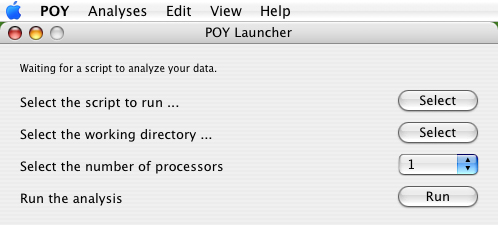
\includegraphics[width=0.75\textwidth]{doc/figures/menu_launcher_window.jpg}
    \end{center}
    \caption{The \poy menu bar and the \emph{POY Launcher} window. These items appear when \poy is opened.}
    \label{fig:menu_launcher_window}
\end{figure}

\subsection{POY menu bar}
The menu bar contains the following drop-down menus:
\begin{description}
%\setlength{\labelwidth}{0pt}
\setlength{\labelsep}{5pt}
\setlength{\itemindent}{0pt}%
\item[POY] (Mac OSX only) contains generic items as with other Mac OSX applications. This pull down menu allows selection of the \emph{About POY} window (Figure~\ref{fig:about_window}) that lists the current version of \poy, a copy write statement, and the address of the \poy website. In addition, it includes a \emph{Quit POY} tab that closes the program. 
\item[Analyses]    contains options for different types of tree searches, calculation of support values, tree diagnosis, and their respective outputs. Other items in this menu open the \emph{POY Launcher} (Open Launcher) and the \emph{Interactive Console}.
\item[Edit] contains standard tools for undoing, cutting, copying, pasting, deleting, and selecting.
\item[View] opens the \emph{Output} window to display the results (including warning and error messages) and the current state of the analysis. 
This \emph{Output} window also contains an \emph{update} tab.  It also contains the \emph{About POY} menu item in Windows and Linux.  
\item[Help] opens the \poy \emph{Manual} in PDF format (requires a PDF viewer).
\end{description}

\begin{figure}[htpb]
    \begin{center}
        
\includegraphics[width=0.5\textwidth]{doc/figures/about_window.jpg}
    \end{center}
    \caption{The \emph{About POY} window.}
    \label{fig:about_window}
        
\end{figure}

\subsection{POY Launcher} 
The \emph{POY Launcher} is the only window that automatically opens upon starting \poy. This allows the user to import a previously created script, designate a working directory, specify the number of processors, and start the analysis.

\begin{description}
%\setlength{\labelwidth}{0pt}
\setlength{\labelsep}{5pt}
\setlength{\itemindent}{0pt}%
	 \item[Select the script to run]
     Allows the user to specify the location of a \poy script.
	\item[Select the working directory]
    The working directory is the
    directory that contains the input data and output files. By default, the working directory is set to be the same as the
    directory containing the selected \poy script. 
	\item[Select the number of processors]
    If more than one computer processor is available, up to 8 cores can be designated for running the analysis. It is important to note that once specified, the selection is applied to \emph{all} subsequent analyses in the current \poy session. The selection of the number of processors is disabled for Linux platforms. Table \ref{ParallelizationGuide} is a guide to the parallelization ability of \poy depending on the operating system and the \poy interface being used. Note that parallelization is \emph{never} supported in interactive sessions, see Section~\ref{interactiveconsole}.
    	\item[Run the analysis]
    Clicking the \emph{Run} button starts the execution of the selected script. Once the script is initiated, the \emph{Run} button
    becomes the \emph{Cancel} button that can be used to interrupt a \poy session.
\end{description}

\begin{table}[t] 
\small
\caption{Parallelization Guide. The field 'mpi+' indicates that mpi must be enabled during compiling. A distinction is made between the interactive console or ncurses that is downloaded from the website (binaries) or that which is compiled from the source.}
\label{ParallelizationGuide} 
\begin{center}
\renewcommand{\arraystretch}{1.5}
\begin{tabular}{p{3.0cm}  p{1.0cm}  p{2.75cm}  p{2.75cm}  p{1.0cm}} 
\hline
	Operating System & GUI & Interactive Console (binaries) & Interactive Console (source) & Flat \\
\hline
	Mac OSX & + & - & - & mpi+ \\
	Windows & + & - & - & mpi+ \\
	Linux & - & - & - & mpi+ \\
\hline
\end{tabular}
\end{center}
\end{table}

If the \emph{Run} button is clicked without the selected script and
working directory, or the names of the scripts and working directory are entered incorrectly, \poy issues an
error message in the upper part of the \emph{POY Launcher} window,
such as \texttt{POY finished with an error}. %l{If nothing is selected and you just hit run, the error output needs to be changed, as it reads "Attemting to change to directory Select or to 'Select' failed misserably. I am cancelling this run, check your path." Attempting, miserable and canceling are misspelled.

\subsection{The \emph{Analyses} menu}
The \emph{Analyses} menu is the main toolbox of the \poy GUI interface (Figure~\ref{fig:simple_search_window}, left). Selections are subdivided into four functional categories. The first three deal with tree searching, support calculation, and tree diagnosis; the fourth one is used for  script management or interactive command execution that bypasses the menu-driven script generating. Each of the menu items is described below in the order it appears on the menu.

Most options are consistently applied through different kinds of analysis. Therefore, all options are described in detail only for the \emph{Simple Search} analysis. The descriptions of other analyses are made with reference to the the \emph{Simple Search} and focus on unique options.

%%%%%%%%%%%
%Tree search options
%%%%%%%%%%%

\subsubsection{Tree searching options}

A number of different tree searching options are available through the \emph{Graphical User Interface}.  These include a \emph{Simple Search}, \emph{Timed Search}, \emph{Search with Ratchet} and \emph{Search with Perturb}.

\subsubsection*{\emph{Simple Search}}
The \emph{Simple Search} window permits the analysis of a number of different data types, including a range of molecular characters (from DNA sequences to whole genomes), custom alphabet characters, and qualitative characters, under parsimony.  It is also possible to carry out a likelihood analysis of DNA sequence data under a number of different models.  
%In the most simplest sense, a typical search involves a series of steps. First, initial trees are generated by random addition sequence from the imported character data. These trees are then subjected to branch swapping, subsequent to which a subset of trees is selected for the report.
The \emph{Simple Search} window (Figure~\ref{fig:simple_search_window}, right) provides the most common and basic options for a standard tree search in \poy that must either (in some cases or) be selected by clicking appropriate buttons or typed. Note that \emph{all the empty fields must be filled in}, otherwise the default values will be used. The window is subdivided into five sections: 

\begin{figure}
\centering
\begin{minipage}[c]{0.45\textwidth}
   		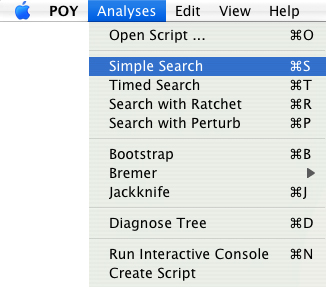
\includegraphics[width=\textwidth]{doc/figures/simplesearch_menu.jpg}
\end{minipage}
\,
\begin{minipage}[c]{0.52\textwidth}
	   	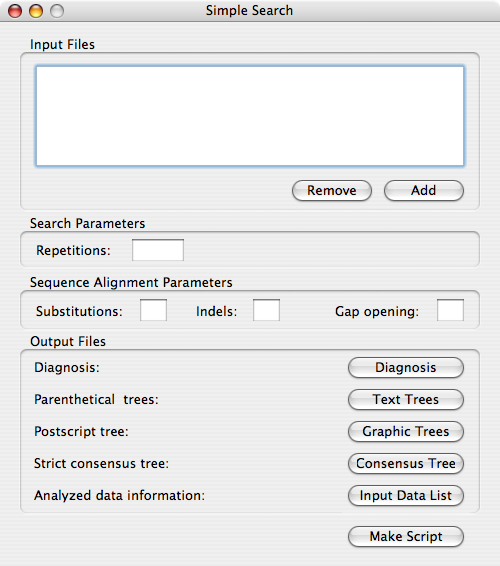
\includegraphics[width=\textwidth]{doc/figures/simplesearch_window.jpg}
   	\end{minipage}
	
\caption{The \emph{Simple Search} window. Selecting \emph{Simple Search} from the \emph{Analysis} menu (left) opens the \emph{Simple Search} window options (right).}
\label{fig:simple_search_window}
\end{figure}

\begin{description}
%\setlength{\labelwidth}{0pt}
\setlength{\labelsep}{5pt}
\setlength{\itemindent}{0pt}%
    \item[Input Files]
        Contains the list of files that are to be input into \poy. These include
        character files in nucleotide, Hennig86, and Nexus formats as well as tree files. (Character data in other formats can be input by specifying additional arguments in the script. See \ccross{read}.) Note: If a Nexus file is input, a gap-opening cost can not be specified, as gaps are independent in this file format.
    \item[Input Parameters]
    	Holds fields to specify the optimality criterion (parsimony or likelihood), the datatype (sequence, break inversion, chromosome, custom alphabet, genome or qualitative) and whether these data types should be treated as prealigned (if possible).  Qualitative data are any non-sequence, prealigned data type (e.g. morphological, behavioral).  These character types are optimized as additive, non-additive or Sankoff characters.
    \item[Sequence Parameters]
        Holds fields to specify the substitution, indel, and gap opening costs. Enter \texttt{0} if no
        gap opening cost is desired. If the value of a parameter is not specified, the default values are used. The default value for both substitutions and insertion deletion events is 1. Within Sequence Parameters an additional subsection is invoked depending on the character type.  \hl{This subsection relates to the costs associated with ....}\\
        Break Inversion Parameters: 	Locus Inversion Cost: default 10\\
        							Level: default 2\\
        Chromosome: 	Locus Breakpoint Cost/Locus Inversion Cost: default 10\\
        				Locus Indel Opening Cost: default 10\\
				Locus Indel Exte\\
        
    \item[Search Parameters]
        Holds one field to set the number of independent random addition replicates to be generated.
    \item[Output Files]
        Designates the names and locations of files containing different kinds of results of the analysis. 
By default, all of these output options are generated, with default names applied.  The names can then be changed 
in the generated script or the option can be removed entirely.  As implied by their respective titles, the \emph{tree} 
buttons output trees in both parenthetical and postscript form.
        \hl{Need to give descriptions of output files here, diagnosis and analyzed data information are not intuitive.
        Also, the different output buttons generate a file, but this is not saved in the script}
\end{description}

\begin{figure}
\centering
\begin{minipage}[c]{0.45\textwidth}
   		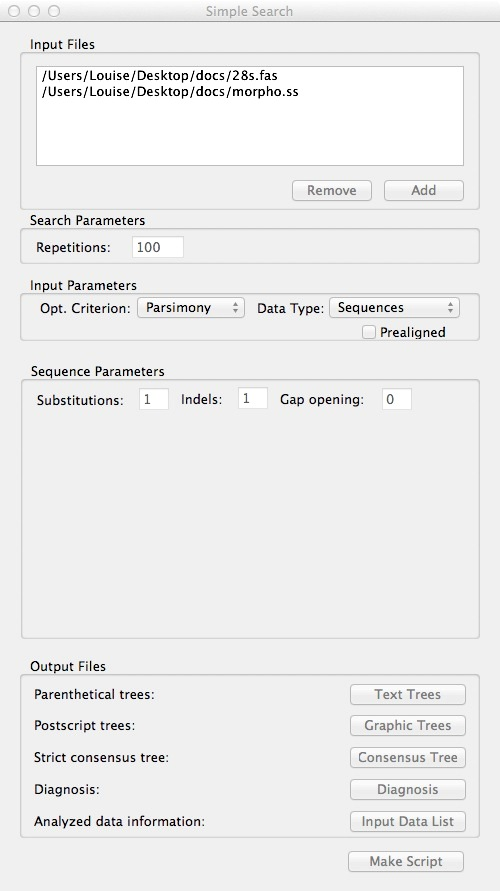
\includegraphics[width=\textwidth]{doc/figures/simplesearch_window_filled.jpg}
\end{minipage}
\,
\begin{minipage}[c]{0.52\textwidth}
	   	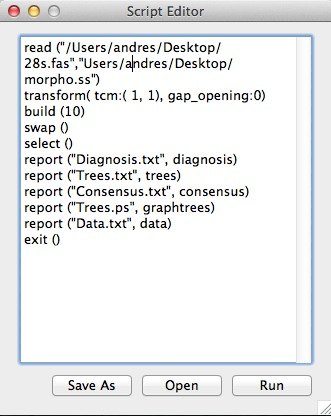
\includegraphics[width=\textwidth]{doc/figures/simplesearch_script.jpg}
   	\end{minipage}
	
    \caption{The \emph{Simple Search} window with specified search parameters and output files (left) and the corresponding \emph{Script Editor} window.}
    \label{fig:ScriptEditor_Window}
\end{figure}

Once all the parameters are selected, click the \emph{Make Script} button and another
window--the \emph{Script Editor}--containing the generated script, appears on screen (Figure~\ref{fig:ScriptEditor_Window}). 
The script can be edited by typing in the commands directly in the \emph{Script Editor} window,
 saved (by clicking the \emph{Save As} button), or replaced with another script (using 
 the \emph{Open} button). To start the analysis, click the \emph{Run} button in the 
 \emph{Script Editor} window. When the \emph{Run} button is clicked, \poy will issue a
 request to save the script. Thus, not only does \poy execute the script but
 it also creates the record of the type of analysis (including all user-defined specifications) that was performed.
 
\subsubsection*{\emph{Timed Search}}

{\emph{Timed Search} (Figure~\ref{fig:timed_search})\hl{ implements a default search strategy that effectively combines tree building with TBR branch swapping, parsimony ratchet, and tree fusing.  The \emph{Timed Search} window has the same four parameter groups described for the \emph{Simple Search}. However, the \emph{Search Parameters} section (called \emph{Search and Perturb Parameters}) contains four fields specifying the search targets instead of the \emph{Repetitions} field. These include the following:}

\begin{figure}
\centering
\begin{minipage}[c]{0.45\textwidth}
   		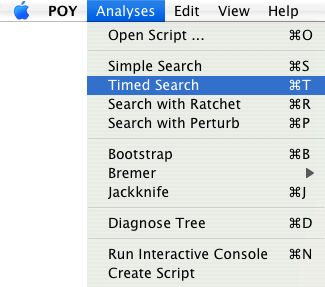
\includegraphics[width=\textwidth]{doc/figures/timedsearch_menu.jpg}
\end{minipage}
\,
\begin{minipage}[c]{0.52\textwidth}
	   	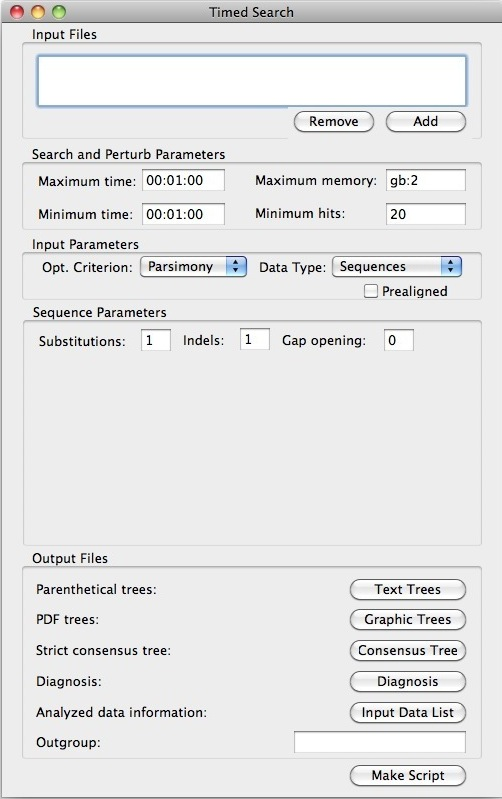
\includegraphics[width=\textwidth]{doc/figures/timedsearch_window.jpg}
   	\end{minipage}
	
\caption{The \emph{Timed Search} window. Selecting \emph{Timed Search} from the \emph{Analysis} menu (left) and viewing the \emph{Timed Search} window options (right).}
\label{fig:timed_search}
\end{figure}

\begin{description}
%\setlength{\labelwidth}{0pt}
\setlength{\labelsep}{5pt}
\setlength{\itemindent}{0pt}%
    \item[Maximum time] The maximum total execution time for the search. The time is specified as
        days:hours:minutes.
    \item[Minimum time] The minimum total execution time for the search. The time is specified as
        days:hours:minutes.
    \item[Maximum memory] The maximum amount of memory allocated for the search.
    \item[Minimum hits] The minimum number of times that the minimum cost must be reached before aborting the search.
\end{description}

This heuristic search is a powerful tool for analyzing data. The number of rounds of successive searching is limited only by the previously mentioned search targets. Therefore, when performing a \emph{Timed Search}, it is crucial to set the maximum time such that the program has a reasonable amount of time to perform a search.  Thus, it is important to have some approximation as to the length of time it would take to perform a single round of searching (e.g. build (1), followed by TBR, ratchet and fusing in the case of a parsimony analysis of DNA sequence data).  Clearly, this is data and optimality criterion dependent.  With this information at hand, the user can then estimate the amount of time necessary to perform a thorough search.  (The user should also allow some time for the program to collate and write the results to files.  If the user opted to run this analysis in parallel, this can take a considerable amount of time.)

\subsubsection*{\emph{Search with Ratchet}}

The parsimony ratchet is a heuristic strategy to escape the local optima during tree searching~\cite{Nixon1999}. The ratchet reweights a given percentage of characters for a specified number of iterations of a search. An analysis is then performed and the resulting tree topology is evaluated using the original data matrix with all characters equally weighted to determine the length of the tree. The \emph{Search with Ratchet} (Figure~\ref{fig:search_with_ratchet_window}) follows the same basic steps of a simple search but includes the ratchet step after the swap. In addition to the same sequence alignment and search parameters as described for the \emph{Simple Search} window, the \emph{Search Parameters} section provides the following ratchet parameters fields:

\begin{description}
%\setlength{\labelwidth}{0pt}
\setlength{\labelsep}{5pt}
\setlength{\itemindent}{0pt}%
    \item[Ratchet iterations] The number of iterations for the parsimony
        ratchet.
    \item[Severity] The severity parameter of the parsimony ratchet (the weight
        change factor for the selected characters).
    \item[Percentage] The percentage of characters to be reweighted during ratcheting.
\end{description}

\begin{figure}
\centering
\begin{minipage}[c]{0.45\textwidth}
   		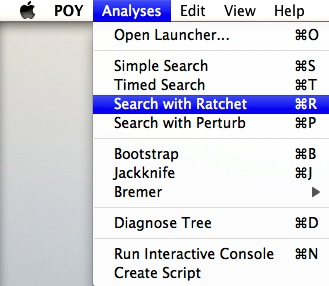
\includegraphics[width=\textwidth]{doc/figures/searchwithratchet_menu.jpg}
\end{minipage}
\,
\begin{minipage}[c]{0.52\textwidth}
	   	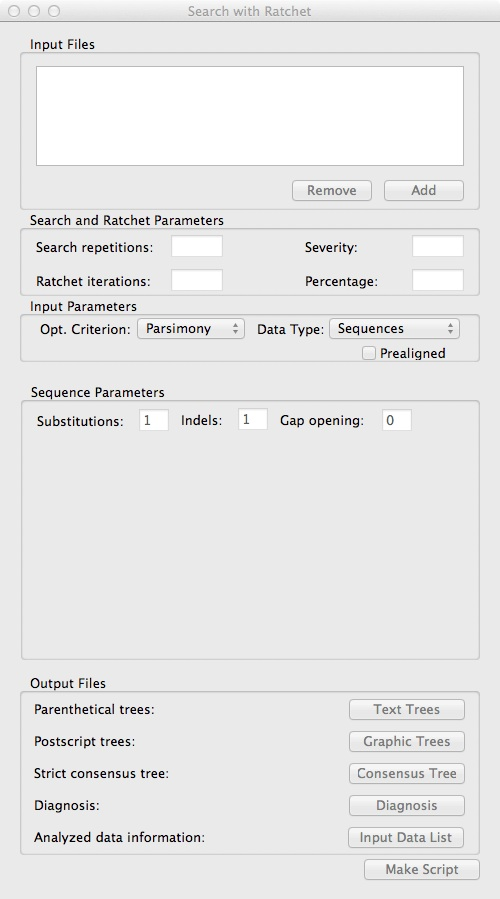
\includegraphics[width=\textwidth]{doc/figures/searchwithratchet_window.jpg}
   	\end{minipage}
	
\caption{The \emph{Search with Ratchet} window. Selecting \emph{Search with Ratchet} from the \emph{Analysis} menu (left) and viewing the \emph{Search with Ratchet} window options (right).}
\label{fig:search_with_ratchet_window}
\end{figure}

\subsubsection*{\emph{Search with Perturb}}

\emph{Search with Perturb} (Figure~\ref{fig:search_with_perturb_window}) provides an alternative means to escape local optima by changing the transformation cost matrix of the molecular characters, a procedure similar in spirit to the parsimony ratchet. In addition to the same sequence alignment and search parameters as described for the \emph{Simple Search} window, the \emph{Search with Perturb} window provides three extra fields with the parameters for the
transformation cost matrix perturbation as follows:

\begin{figure}
\centering
\begin{minipage}[c]{0.45\textwidth}
   		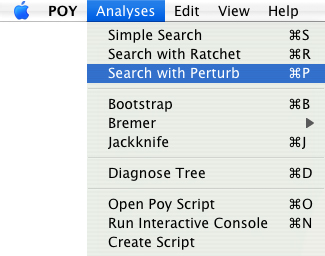
\includegraphics[width=\textwidth]{doc/figures/searchwithperturb_menu.jpg}
\end{minipage}
\,
\begin{minipage}[c]{0.52\textwidth}
	   	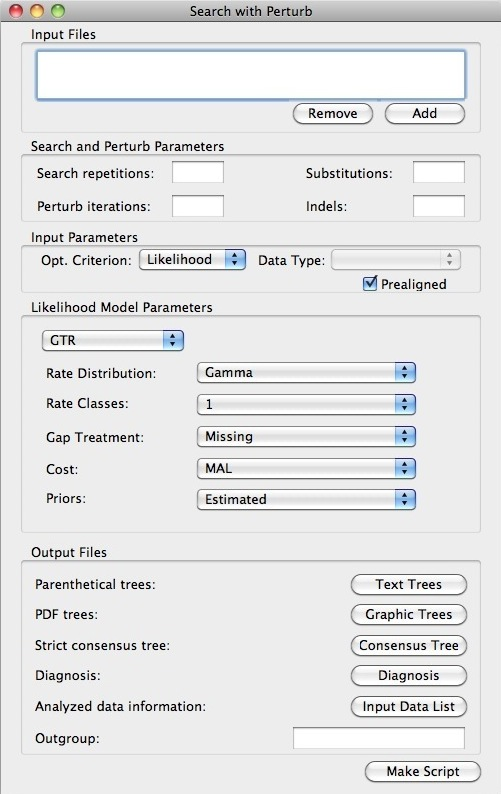
\includegraphics[width=\textwidth]{doc/figures/searchwithperturb_window.jpg}
   	\end{minipage} 
\caption{The \emph{Search with Perturb} window. Selecting \emph{Search with Perturb} from the \emph{Analysis} menu (left) and viewing the \emph{Search with Perturb} window options (right).}
\label{fig:search_with_perturb_window}
\end{figure}

\begin{description}
%\setlength{\labelwidth}{0pt}
\setlength{\labelsep}{5pt}
\setlength{\itemindent}{0pt}%
    \item[Perturb iterations] Sets the number of perturb iterations to be performed.
    \item[Substitutions] Specifies the cost of the perturbed substitutions.
    \item[Indels] Specifies the cost of the perturbed indels.
\end{description}

During this heuristic search, \poy performs a parsimony ratchet search during each iteration (default values are used, i.e. 25\% probability, 2 severity).

\subsubsection{Support calculation options}

It is possible to calculate different support values using this interface.  Two of these measures, Bootstrap and Jackknife, involve resampling techniques, while the third, Bremer support, is an optimality-based measure based on the cost of the tree. 

None of the support calculation windows include functions for tree building and searching. Therefore, one of the input files must contain trees for which support values are going to be calculated. \hl{Put jackknife before bremer}

\subsubsection*{\emph{Bootstrap}}

As a resampling technique, the non-parametric \emph{Bootstrap} resamples the original data, creating a simulated dataset equal to the size of the original dataset.  The characters are replaced in between each iteration. The \emph{Bootstrap} window (Figure~\ref{fig:bootstrap}) specifies parameters for estimating the Bootstrap support values. In addition to the \emph{Simple Search} window fields, it contains a a field for the bootstrap parameters, in this case a \emph{Pseudoreplicates} field, to specify the number of bootstrap pseudoreplicates.

\begin{description}
%\setlength{\labelwidth}{0pt}
\setlength{\labelsep}{5pt}
\setlength{\itemindent}{0pt}%
    \item[Pseudoreplicates] Specifies the number of resampling iterations.
\end{description}

\begin{figure}
\centering
\begin{minipage}[c]{0.45\textwidth}
   		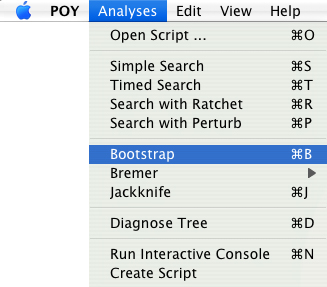
\includegraphics[width=\textwidth]{doc/figures/bootstrap_menu.jpg}
\end{minipage}
\,
\begin{minipage}[c]{0.52\textwidth}
	   	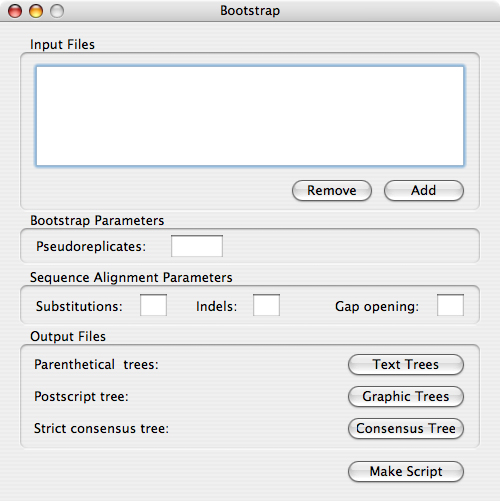
\includegraphics[width=\textwidth]{doc/figures/bootstrap_window.jpg}
   	\end{minipage}
\caption{The \emph{Bootstrap} window. Selecting \emph{Bootstrap} from the \emph{Analysis} menu (left) and viewing the \emph{Bootstrap} window options (right).}
\label{fig:bootstrap}
\end{figure}

\subsubsection*{\emph{Jackknife}}

An alternative statistical measure of support is the \emph{Jackknife}, wherein the original data matrix is resampled, but in this case without replacement.  The \emph{Jackknife} window (Figure~\ref{fig:jackknife}) specifies parameters for estimating the
Jackknife support values. In addition to the \emph{Simple Search} window fields, \emph{Jackknife Parameters} contains fields to specify
the number of Jackknife pseudoreplicates (\emph{Pseudoreplicates}) and the number of characters to be removed (\emph{Remove}) during each pseudoreplicate.

\begin{figure}
\centering
\begin{minipage}[c]{0.45\textwidth}
   		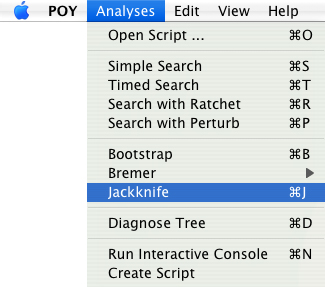
\includegraphics[width=\textwidth]{doc/figures/jackknife_menu.jpg}
\end{minipage}
\,
\begin{minipage}[c]{0.52\textwidth}
	   	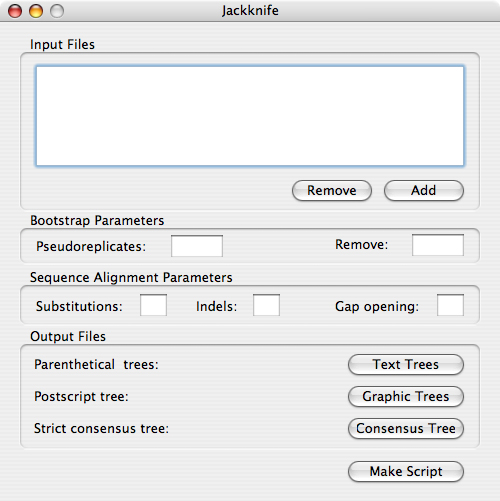
\includegraphics[width=\textwidth]{doc/figures/jackknife_window.jpg}
   	\end{minipage}
\caption{The \emph{Jackknife} window. Selecting \emph{Jackknife} from the \emph{Analysis} menu (left) and viewing the \emph{Jackknife} window options (right).}
\label{fig:jackknife}
\end{figure}

\begin{description}
%\setlength{\labelwidth}{0pt}
\setlength{\labelsep}{5pt}
\setlength{\itemindent}{0pt}%
    \item[Pseudoreplicates] Specifies the number of resampling iterations.
    \item[Remove] Specifies the percentage of characters being deleted during a pseudoreplicate.
\end{description}

\subsubsection*{\emph{Bremer}}

The \emph{Bremer} option (Figure~\ref{fig:search_for_bremer_menu}) is divided into two windows: the \emph{Search for Bremer} window, that specifies the Bremer support \cite{Bremer1988, Kallersjoetal1992} calculation parameters, and the \emph{Report Bremer} window to format the output of the results (Figure~\ref{fig:search_report_bremer}). 

\paragraph{Search for Bremer}

\begin{figure}[htpb]
    \begin{center}
        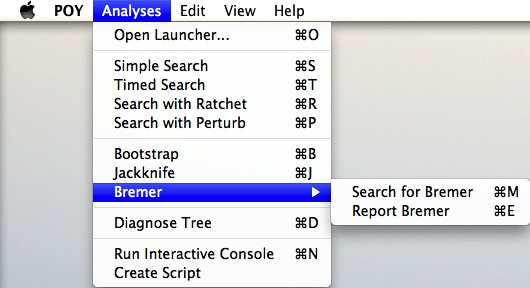
\includegraphics[width=0.65\textwidth]{doc/figures/searchforbremer_menu.jpg}
    \end{center}
    \caption{ Selecting the \emph{Bremer} windows from the \emph{Analysis} menu.}
    \label{fig:search_for_bermer_menu}
\end{figure}

\begin{figure}
\centering
\begin{minipage}[c]{0.45\textwidth}
   		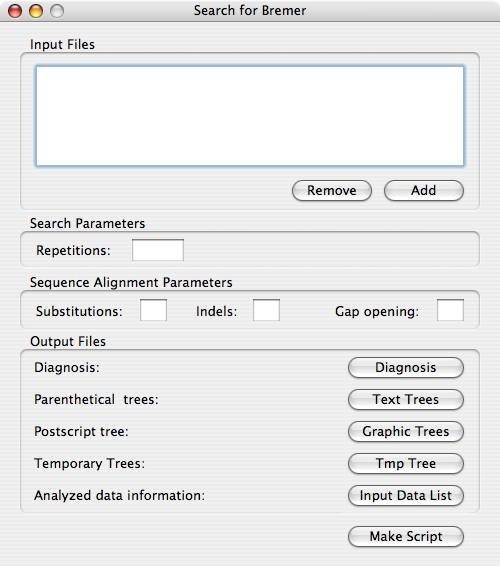
\includegraphics[width=\textwidth]{doc/figures/searchforbremer_window.jpg}
\end{minipage}
\,
\begin{minipage}[c]{0.52\textwidth}
	   	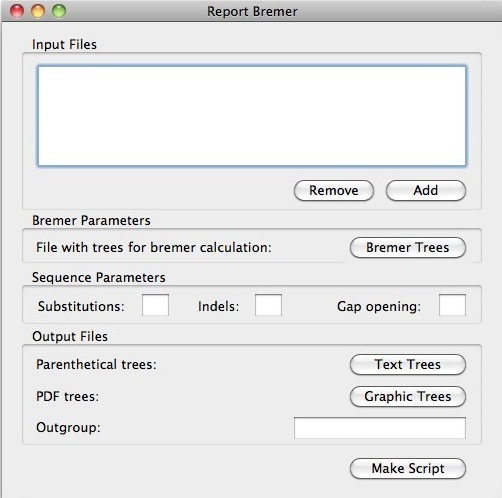
\includegraphics[width=\textwidth]{doc/figures/reportbremer_window.jpg}
   	\end{minipage}
\caption{Viewing the options of the \emph{Search for Bremer} (left) and the \emph{Report Bremer}(right) windows.}
\label{fig:search_report_bremer}
\end{figure}

The script produced in this window collects trees visited during a search for Bremer support calculations. This
search can take a long time, as the goal of this search strategy is to broadly sample variation among trees, and guarantee that all
clades have Bremer support values. 

In addition to the standard four sections defined for the \emph{Simple Search} window,
note that one of the output files is the \emph{Temporary Trees} file, which 
contains all the information required to produce the bremer support tree
results in the \emph{Report Bremer} window. Make sure to choose a file name that does not overwrite this output.

If the search does not finish within the time frame amenable to the user the search can be interrupted and the intermediate results remain stored in the \emph{Temporary Trees} file.  As Bremer calculations are upper-bound values, terminating the search prior to completion and, thus, storing a smaller pool of visited trees may inflate support values relative to those generated by a more exhaustive search. The trees from the \emph{Temporary Trees} file can then be reported using the \emph{Report Bremer} window.

\paragraph{Report Bremer}
The script produced in this window takes the \emph{Temporary Trees} file generated in the \emph{Search for Bremer} window in the \emph{File with trees for bremer calculation} field. 

\subsubsection{Diagnosis}

\subsubsection*{\emph{Diagnose Tree}}

The \emph{Diagnose Tree} window (Figure~\ref{fig:diagnosetree}) specifies parameters for reporting a diagnosis of the input tree. This window lacks the \emph{Search Parameters} section because the diagnosis is performed on the trees resulted from prior searches and no new trees are generated during the diagnosis procedure. \hl{It is important to add both the input tree (or trees?) in addition to the data file in order to diagnose the tree.  The costs of the tree can be changed here.}

\begin{figure}
\centering
\begin{minipage}[c]{0.45\textwidth}
   		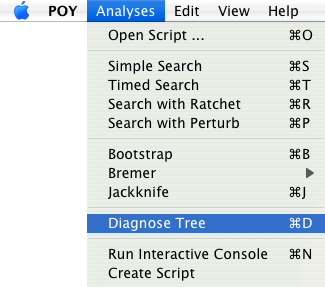
\includegraphics[width=\textwidth]{doc/figures/diagnose_menu.jpg}
\end{minipage}
\,
\begin{minipage}[c]{0.52\textwidth}
	   	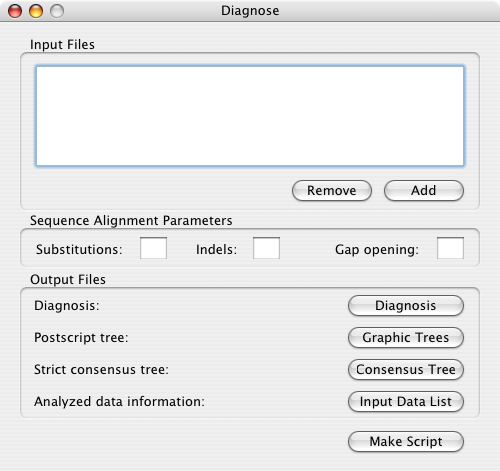
\includegraphics[width=\textwidth]{doc/figures/diagnose_window.jpg}
   	\end{minipage}
\caption{The \emph{Diagnose} window. Selecting \emph{Diagnose Tree} from the \emph{Analysis} menu (left) and viewing the \emph{Diagnose} window options (right).}
\label{fig:diagnosetree}
\end{figure}

\subsubsection{\emph{Script editing and the Interactive Console}}

\subsubsection*{Open POY Launcher}

Selecting \emph{Open POY Script} (Figure~\ref{fig:open_poy_script}) displays the \emph{POY Launcher} 
window (Figure~\ref{fig:menu_launcher_window}), the function of which is described above.

\begin{figure}[htpb]
    \begin{center}
        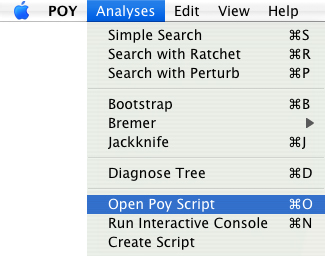
\includegraphics[width=0.5\textwidth]{doc/figures/openpoyscript_menu.jpg}
    \end{center}
    \caption{The \emph{Open POY script} selection opens the \emph{POY Launcher} window.}
    \label{fig:open_poy_script}
\end{figure}

\subsubsection*{Run Interactive Console}

Selecting \emph{Run Interactive Console} (Figure~\ref{fig:runinteractive}) opens the ncurses interface
that enables the user to run the analysis interactively by entering \poy commands directly via the command-line interface of the \emph{Interactive Console} See \emph{Using the Interactive Console} (Section \ref{interactiveconsole}).

\begin{figure}
\centering
\begin{minipage}[c]{0.45\textwidth}
   		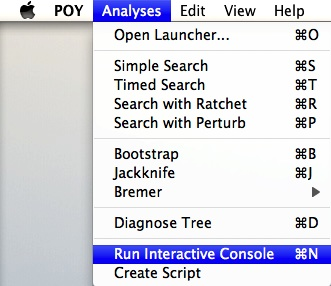
\includegraphics[width=\textwidth]{doc/figures/runinteractive_menu.jpg}
\end{minipage}
\,
\begin{minipage}[c]{0.52\textwidth}
	   	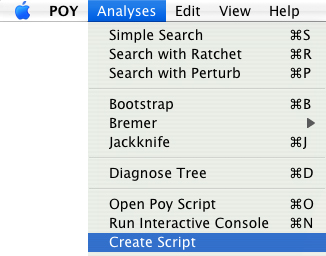
\includegraphics[width=\textwidth]{doc/figures/create_script_window.jpg}
   	\end{minipage}
\caption{The \emph{Run Interactive Console} selection (left) opens \poy interactive console in a new window. The \emph{Create Script} selection opens the \emph{Script Editor} window (Figure~\ref{fig:ScriptEditor_Window}).}
\label{fig:runinteractive}
\end{figure}

\subsubsection*{Create Script}
The \emph{Create Script} selection opens a blank \emph{Script Editor} window that allows opening, creating, modifying, saving, and executing  a customized script.

\subsection{The \emph{View} menu}

The \emph{View} menu contains the \emph{Output} window which is subdivided into two fields: the upper \emph{Results and Errors} and lower \emph{Status of Search} (Figure~\ref{fig:results_and_status_windows}). These fields display, respectively, the results (including warning and error messages) and the current state of the analysis. These fields are not updated automatically and in order to display the current state of the analysis the user must click the \emph{Update} button. The \emph{View} menu also contains the \emph{About POY} window in Windows and Linux.

\begin{figure}
\centering
\begin{minipage}[c]{0.45\textwidth}
   		
\includegraphics[width=\textwidth]{doc/figures/view_menu.jpg}
\end{minipage}
\,
\begin{minipage}[c]{0.52\textwidth}
	   	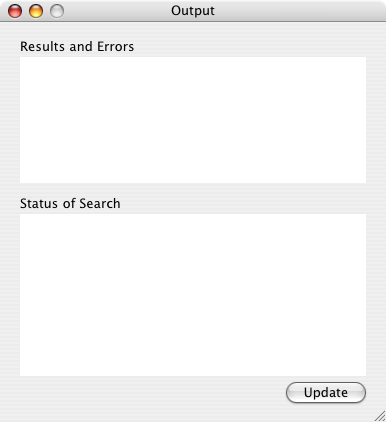
\includegraphics[width=\textwidth]{doc/figures/output_window.jpg}
   	\end{minipage}
\caption{Selecting the \emph{Output} window (left) and viewing the \emph{Results and Errors} and  \emph{Status of Search} fields.}
\label{fig:results_and_status_windows}
\end{figure}

%%%%%%%%%%%%%%%%%%%%%%%%%%%%%%%%%%%%%%%%%%%%%%%%%%%%%%%%%%%%%%%%%%
%INTERACTIVE CONSOLE%
%%%%%%%%%%%%%%%
\section{Using the Interactive Console} \label{interactiveconsole}

This section will help you get started using the \poy \emph{Interactive Console} and will prepare you for the
more extensive, technical descriptions in the next chapter, \emph{\poy Commands}. %Now that you are acquainted with the program's interface, learned how to initiate, and exit or interrupt a \poy session, you are well prepared to run your first analysis.%
This section will teach you how to input data files, check the data you are analyzing, generate a set of initial trees, do basic branch swapping to find a local optimum, and, finally, produce and visualize the resultant trees, their strict consensus, and generate support values in a command-line environment rather than using a \emph{Graphical User Interface}. 

For the purpose of this exercise, three data files are used available at \\
\begin{center}
\url{http://research.amnh.org/scicomp/projects/poy.php}
\end{center}

\begin{itemize}
	\item {\texttt{18s.fas} and \texttt{28s.fas} contain unaligned DNA sequences (partial 18S and 28S ribosomal DNA) in FASTA format.~\cite{pearson1988}}
	\item {\texttt{morpho.ss} contains a morphological data matrix in Hennig86 format.~\cite{farris1988}}
\end{itemize}

Once \poy has been launched and the interface (Figure~\ref{fig:figinterface}) had appeared on the screen, the data can be input and the analysis can proceed. As you follow the instructions, you are encouraged to consult the help file by using the command \commandstyle{help} (see Section~\ref{sec:help} to learn more about \poy commands and their arguments).

\subsection{The interface}

The \emph{Interactive Console} provides a terminal environment with enhanced ability to display the results and the state of the analysis. It is recommended to use the console to explore and verify the data in the early steps of the analysis, and to learn the scripting language. \hl{As opposed to what? I'd imagine that a lot of people will never compile and use the flat environment. The only benefit to not using the interactive console and going with flat, is that you can run in parallel or a cluster} Using the console requires familiarity with \poy commands, their arguments, and the conventions of \poy scripting (which are discussed in the \emph{POY Commands} chapter). It has four windows: \emph{POY Output}, \emph{Interactive Console}, \emph{State of Stored Search}, and \emph{Current Job} (Figure \ref{fig:figinterface}):

\begin{figure}[htbp]
   \centering
   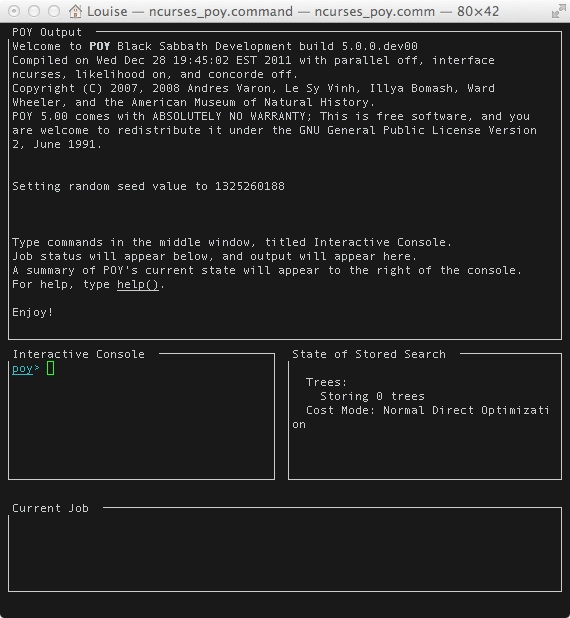
\includegraphics[width=0.7\textwidth]{doc/figures/figinterface.jpg}
   \caption{\poy interface displayed in the Terminal window prior to analysis. Note the cursor at the \poy prompt in the \emph{Interactive Console} and that the \emph{State of Stored Search} and \emph{Current Job} windows are empty.}
   \label{fig:figinterface}
\end{figure}

\begin{description}
%\setlength{\labelwidth}{0pt}
\setlength{\labelsep}{5pt}
\setlength{\itemindent}{0pt}%
\item[POY Output] (Figure \ref{fig:figinterface}, upper box) displays the status of the imported data, outputs the results of the phylogenetic analyses (such as trees, character diagnoses, and implied alignments), reports errors, and displays descriptions of \poy commands.
\item[Interactive Console] (Figure \ref{fig:figinterface}, mid-left box) is used to issue the commands interactively and to execute the commands by clicking the Return key. (See Section~\ref{commands} on the description of \poy commands.)
\item[State of Stored Search] (Figure \ref{fig:figinterface}, mid-right box) displays the time (in seconds) elapsed since the initiation of the current operation. This window also reports the number of trees currently in memory and displays the range of their costs.
\item[Current Job] (Figure \ref{fig:figinterface}, lower box) describes the currently running operation. When the operation is completed, the box is blank.
\end{description} 

\begin{figure}[htbp]
   \centering
   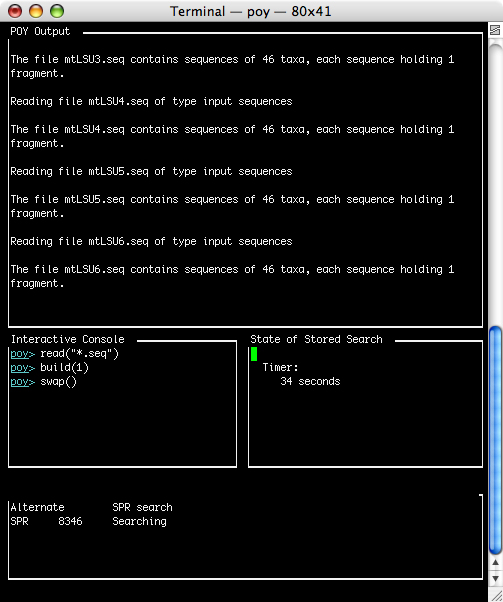
\includegraphics[width=0.7\textwidth]{doc/figures/figprocess.jpg}
   \caption{\poy interactive console during a process. The \emph{POY Output} window displays (by default) the information on the input data files. The \emph{Interactive Console} lists the commands that have been consecutively executed. The \emph{Current Job} window shows the state of the current operation and the current tree score. The \emph{State of Stored Search} shows the time elapsed  since the last command, \commandstyle{swap}, was initiated.}
   \label{fig:figprocess}
\end{figure}

%This \poy interface is not available for parallel environments. Once the program is invoked, \poy commands can be executed interactively or scripts can be submitted as when using the \emph{Interactive Console}. By default, \poy will print the output to screen (the same output that is reported in \emph{POY Output} under non-parallelized setting).


\subsection{Starting a \poy session using the \emph{Interactive Console}}

\begin{flushleft}
	\begin{minipage}[c]{0.074\textwidth}
	   	
\includegraphics[width=\textwidth]{doc/figures/figlogowindows.jpg}
	\end{minipage}
	\,
	\begin{minipage}[t]{0.88\textwidth}
		\subsubsection*{Windows}
	\end{minipage}
			\begin{itemize}
                \item{Start$>$All Programs$>$POY$>$Interactive Console}
			\end{itemize}

	\begin{minipage}[c]{0.074\textwidth}
   		
\includegraphics[width=\textwidth]{doc/figures/figlogomac.jpg}
	\end{minipage}%
	\,
	\begin{minipage}[t]{0.88\textwidth}
	   	\subsubsection*{Mac OSX}
	\end{minipage}
			\begin{itemize}
				\item {Double-click \poy application icon to start the program.}
				\item {Select \emph{Run Interactive Console} from the
				\emph{Analyses} menu.}
			\end{itemize}		

	\begin{minipage}[c]{0.074\textwidth}
   		
\includegraphics[width=\textwidth]{doc/figures/figlogolinux.jpg}
	\end{minipage}
	\,
	\begin{minipage}[t]{0.88\textwidth}
	   	\subsubsection*{Linux}
	\end{minipage}
	\begin{itemize}
    		\item Add \texttt{/opt/poy4/Resources/} to your \texttt{PATH} and run
    \texttt{ncurses\_poy} from a terminal.
    	\end{itemize}
\end{flushleft}

\subsection{Entering commands}
Once this \poy interface is opened, the cursor appears in the \emph{Interactive Console} portion of the window and is ready to accept commands. The interactive console does not support using the mouse and, as true for most command-line applications, the cursor can be moved using the left and right arrow keys, and the Backspace (in Windows) or Delete (in Mac) keys are used to erase individual characters to the left of the current cursor position. To eliminate the need of retyping commands anew during a \poy session, keyboard shortcuts can be used: control-P (``previous'') and control-N (``next'') will scroll through the commands previously entered during the session. In addition, the interactive console is equipped with the autocomplete feature: it involves \poy predicting a command, an argument, of file name that the user wants to type from the first letter(s) entered. Upon typing the first letter or part of the phrase, repeatedly pressing the TAB key scrolls through the list of command, argument, and file names that begin with that letter or phrase. Autocomplete speeds up interaction with the program.

\subsection{Browsing the output}
As more output is reported in the \emph{POY Output} window, only the most recent reports will be seen in the window. Using the Up and Down keys allows the user to scroll up and down the \emph{POY Output} window to see the welcome line, and previously printed reports and help descriptions. Pressing Up and Down keys automatically places the cursor in the lower left corner of the \emph{POY Output} window indicating that you are interacting with that window. Only 1000 lines are stored in the memory and the output that was reported before that will not be accessible by scrolling. The number of lines, however, can be modified by the user using the command \poycommand{set()}, see~\ccross{history}. If the user desires to keep the entire output or specific items in the output, a log can be created using the command \poycommand{set()}, see~\ccross{log}) or specific outputs can be redirected to files (see~\ccross{report}).  The user should be aware that outputting a log file can slow down the program due to I/O (input/output) delay.

\subsection{Switching between the windows}
To return to the \emph{Interactive Console}, start typing and the cursor will automatically be placed back at the \poy prompt. When an operation is in progress (shown in the \emph{Current Job} window), the cursor stays in the upper left corner of the \emph{State of Current Search} window, and switching between the \emph{Interactive Console} and the \emph{POY Output} window is disabled. There are no user interactions in the \emph{Current Job} or \emph{State of the State of Current Search}.

\subsection{Importing data} \label{sec:import}

The basic command to input data in \poy is \commandstyle{read()}, which includes the list of files (in quotation marks and separated by commas) enclosed in parentheses. Suppose that we would like to simultaneously analyze morphological and molecular datasets, contained in separate data files, \texttt{morpho.ss} and \texttt{28s.fas}, respectively. We can issue a pair of \commandstyle{read()} commands (Figure~\ref{fig:readingexample}):
\begin{quote}
        \commandstyle{read("morpho.ss")}\\
        \commandstyle{read("28s.fas")}
\end{quote}

\begin{figure}
    \begin{center}
        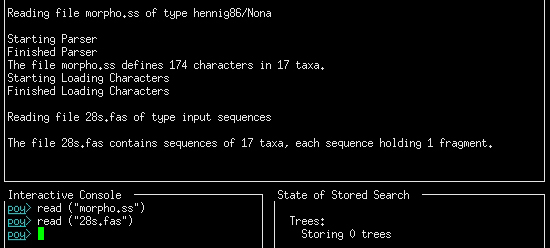
\includegraphics[width=0.7\textwidth]{doc/figures/reading_example.jpg}
    \end{center}
    \caption{Importing data files using the \emph{Interactive Console}. Two consecutive \commandstyle{read} commands specify both the morphological data file in Hennig86 format (\texttt{morpho.ss}), and the molecular data file in FASTA format (\texttt{28s.fas}). Note that \poy automatically reports  in the \emph{POY Output} window the names and types of files that have been imported.}
    \label{fig:readingexample}
\end{figure}

The syntax of \commandstyle{read}, like every command in \poy, contains two elements: the name of the command, in this case \commandstyle{read}, followed by an optional list of arguments 
separated by commas and enclosed in parentheses. All filenames read into \poy should include the appropriate suffix for the file type (e.g. .fas, .ss, .aln, .tre etc:).  Typically, the arguments of the command \commandstyle{read()} are names of data files, each being enclosed in double quotes (as shown in the example above). Even though there might be only one argument or none in some commands, parentheses (e.g. \poycommand{read()}) always follow the command name. An exhaustive discussion of \poy command structure and detailed descriptions of all commands with examples of their usage are provided in the \emph{POY Commands} chapter (\ref{commands}).

In order to import data by entering the names of the files, the directory containing these files must be identified.  This can be established in two ways--by using the command \commandstyle {cd} to redirect the path to the directory where the data is found and then reading in the data file:\\
\begin{quote}
\commandstyle{cd ("/Users/username/docs/poyfiles")}\\
\commandstyle{read ("28s.fas")}\\
\end{quote}
or by including the full path in the argument of \commandstyle{read}:\\
\begin{quote}
\commandstyle{read("/Users/username/docs/poyfiles/28s.fas")}
\end{quote}

Most of the time users are interested in importing multiple data files to analyze an entire dataset. In this case, multiple data files can be specified as arguments for a single command. For example, importing both files, \texttt{morpho.ss} and \texttt{28s.fas}, can be written more succinctly:\\
\begin{quote}
\commandstyle{read("morpho.ss", "28s.fas")}
\end{quote}
or if the full path is included in the argument of \commandstyle{read} as: \\

\begin{quote}
\commandstyle{read("/Users/username/docs/poyfiles/morpho.ss", \\
			"/Users/username/docs/poyfiles/28s.fas")}
\end{quote}

This is equivalent to sequentially importing each file as shown in (Figures ~\ref{fig:readingexample} and \ref{fig:reading_example2}).

Figures~\ref{fig:readingexample} and \ref{fig:reading_example2} also illustrate an important feature that makes \poy different from many other phylogenetic analysis programs: every time a file is imported during a \poy session, the input data are \emph{added} to the current data in memory and \emph{do not replace them}. This allows additional analytical flexibility. For example, if only morphological data are read and trees are built based on these data alone, a subsequently imported molecular character dataset will be used in conjunction with the previously imported morphological data, despite the fact that current trees in memory were generated only from morphological data (Figure~\ref{fig:reading_example2}):

\begin{quote}
\commandstyle{read("morpho.ss")}\\
\commandstyle{build()}\\
\commandstyle{read("28s.fas")}\\
\commandstyle{rediagnose()}\\
\commandstyle{swap()}
\end{quote}

It must be noted that if the numbers of terminals differ among data files, \emph{only} the data that correspond to the terminals used to generate the trees (in this case, the morphological data file) are used. The rest of the character data are ignored, unless the trees are built again with the data files containing the expanded number of terminals.

Also, because \poy appends trees and data in memory, it is a good practice when starting a new analysis to empty the memory using use the command \commandstyle{wipe()}.

\begin{figure}[]
    \begin{center}
        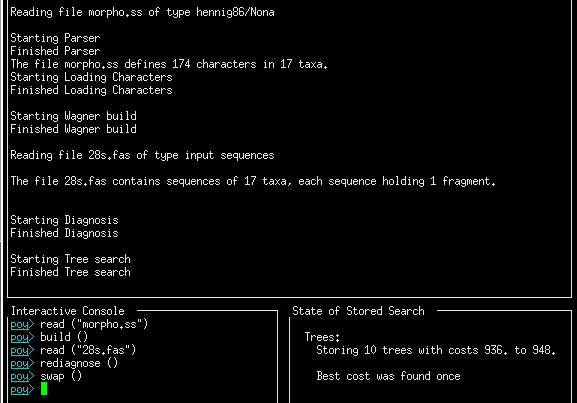
\includegraphics[width=0.6\textwidth]{doc/figures/reading_example2.jpg}
    \end{center}
    \caption{Building trees with morphological data only but continuing analysis using combined morphological and molecular data. This example shows how we can add data to the analysis incrementally by loading files at different points in the search. First, the morphological data are imported from \texttt{morpho.ss} file using \poycommand{read()} the and trees are built based on these data. Then molecular data from the \texttt{28s.fas} file are loaded into memory in addition to previously imported morphological data. Finally, subsequent analyses, \commandstyle{rediagnose()} and \commandstyle{swap()}, are conducted using the data in memory, that is the trees based on morphological data, and both morphological and molecular character sets.}
    \label{fig:reading_example2}
\end{figure}

Valid input files include nucleotide and amino acid sequence files in many formats,
and morphological data in Hennig86 and Nexus formats. (For information on specific formats supported by \poy and other types of input files see \commandstyle{help(read)}.)

\subsection{Inspecting data}

Once a dataset (or multiple datasets) is imported, \poy automatically reports a brief description of contents for each loaded file in the \emph{POY Output} (Figure ~\ref{fig:readingexample}). However, it may be desirable to inspect the imported data in greater detail to ensure that the format and contents of the files have been interpreted correctly. This practice helps to avoid common errors, such as inconsistently spelled terminal names, which may result in bogus results, produce error messages, and aborted jobs.

The basic command for outputting information is \commandstyle{report()}. One of its arguments, \commandstyle{data}, outputs a set of tables showing the list of terminals, the number and types of characters, and the lists of terminals and characters excluded from the analysis. To produce a report of the data files that were used in the previous example (\texttt{morpho.ss} and \texttt{28s.fas}), we import the data and execute \commandstyle{report(data)}:
\begin{quote}
    \commandstyle{read("morpho.ss", "28s.fas")}\\
    \commandstyle{report(data)}
\end{quote}
This will generate an extensive, detailed output, partial views of which are shown in Figure ~\ref{fig:reportdata}. Obviously, the entire report will not be visible in the \emph{POY Output} window. Therefore, the Up and Down arrow keys and Page Up and Page Down keys can be used to scroll.  By default, \poy reports the results of executed commands to the \emph{POY Output} window. However, the same output can be redirected to a file simply by adding the name of the output file in the list of argument of the command \commandstyle{report()} \emph{before} the argument specifying the type of the requested report (in this case \commandstyle{data}, see the command~\ccross{report} ). For instance, if we would like to output into the file ``data\_analyzed.txt,'' we would enter:
\begin{quote}
    \commandstyle{read("morpho.ss", "28s.fas")}\\
    \commandstyle{report("data\_analyzed.txt", data)}
\end{quote}

\begin{figure}
\centering
\begin{minipage}[c]{0.52\textwidth}
   		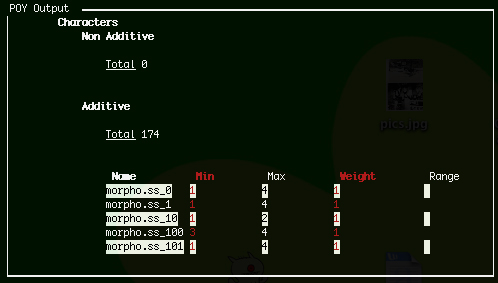
\includegraphics[width=\textwidth]{doc/figures/report2.jpg}
\end{minipage}
\,
\begin{minipage}[c]{0.44\textwidth}
	   	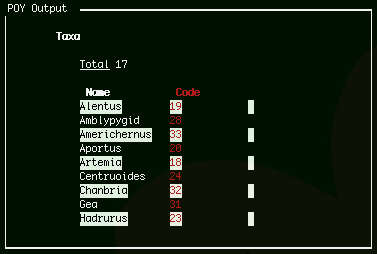
\includegraphics[width=\textwidth]{doc/figures/report3.jpg}
   	\end{minipage}
\caption{Inspecting imported data. The figure shows segments of a data report generated by \commandstyle{report(data)}. The left and right panels demonstrate a typical table output the character and terminal data respectively.}
\label{fig:reportdata}
\end{figure}

In this example, all the imported data are analyzed and, therefore, the report fields that list excluded data will appear empty. One can, however, exclude specific characters or terminals from the analysis using additional commands (see the command~\ccross{report}).

Another useful argument of \commandstyle{report} is \commandstyle{cross\_references}. This argument displays whether character data are present or absent for each terminal in each one of the imported data files. This provides a comprehensive visual overview of missing data. Building on the previous example, such output can be generated by the following sequence of commands:
\begin{quote}
    \commandstyle{read("morpho.ss", "28s.fas")}\\
    \commandstyle{report("cross\_refs.txt", cross\_references)}
\end{quote}

\begin{figure}[]
    \begin{center}
        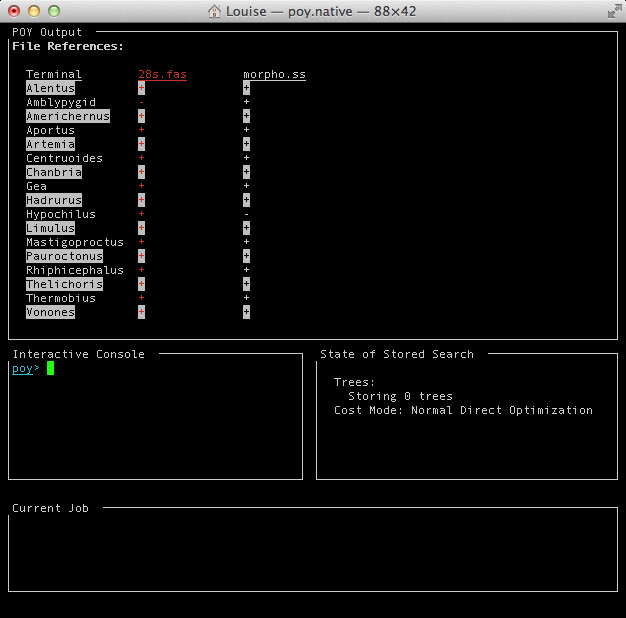
\includegraphics[width=0.6\textwidth]{doc/figures/crossref.jpg}
    \end{center}
    \caption{Visualizing missing data. The command \commandstyle{cross\_references} displays a table showing whether a given terminal (in the left column) is present (``+'') or absent (``-'') in each data file. In this example, \texttt{28s.fas} is missing for Amblypygid and \texttt{morpho.ss} for Hypochilus.}
    \label{fig:crossref}
\end{figure}

A typical output of \commandstyle{cross\_references} command is shown in Figure ~\ref{fig:crossref}.

\subsection{Building the initial trees}

The command to build trees is \commandstyle{build()} (already mentioned in Section~\ref{sec:import}). After importing \texttt{morpho.ss} and \texttt{28s.fas}, executing the command \commandstyle{build()} without specifying any arguments (default settings) generates 10 trees by random addition sequence.

Many \poy commands operate under default settings when executed without arguments. To learn what the default settings are for a particular command, use either \commandstyle{help()} command with the command name of interest inserted in parentheses or consult the \emph{POY Commands} chapter (\ref{commands}).

If the user would like to specify a number of tree building replicates different from the default value of 10, an argument \commandstyle{trees} followed by a colon (``:'') and an integer specifying the number of trees must be included in the argument list of the \commandstyle{build} command: \commandstyle{build(trees:100)}. This command has a shortcut that omits the argument \commandstyle{trees}. Thus, \commandstyle{build(trees:100)} is equivalent to \commandstyle{build(100)}. As defaults, the shortcuts are fully described in Section \ref{commands}. The entire sequence of commands minimally required to import the data and build 100 trees is the following:

\begin{quote}
 	\commandstyle{read("morpho.ss","28s.fas")}\\
 	\commandstyle{build(100)}
\end{quote}

As the tree building advances, the \emph{Current Job} window displays the current status of the operation (Figure~\ref{fig:building}). This window shows how many Wagner builds have been performed out of the total number requested, the number of terminals added in the current build, the cost of the current tree (recalculated after each terminal addition), and the estimated time for the completion of all the builds. When all the trees are generated, the \emph{State of Stored Search} window displays the range of tree costs (the best and worst costs), the number of trees stored in memory, and the number of trees with the best cost (Figure~\ref{fig:building}).

\begin{figure}
\centering
\begin{minipage}[c]{0.507\textwidth}
   		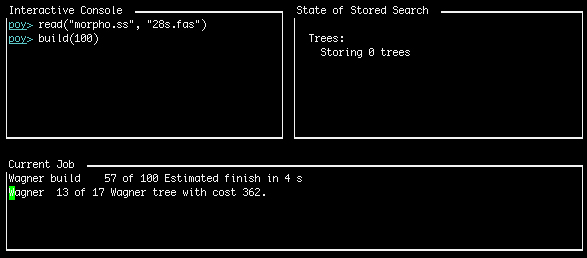
\includegraphics[width=\textwidth]{doc/figures/building1.jpg}
\end{minipage}
\quad
\begin{minipage}[c]{0.453\textwidth}
	   	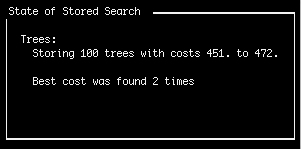
\includegraphics[width=\textwidth]{doc/figures/building2.jpg}
   	\end{minipage}
\caption{Generating Wagner trees. During the process of tree building (left panel), the \emph{Current Job} window displays how many builds have been performed so far (\texttt{57 of 100}), the number of terminals added in the current build (\texttt{13 of 17}), a cost of a current tree recalculated after each terminal addition (\texttt{362}), and the estimated time (in seconds) for the completion of the operation (\texttt{4 s}). Because the process is not complete, the \emph{State of Stored Search} window contains no trees. Once tree building is complete, the \emph{State of Stored Search} window displays the best (\texttt{451}) and worst (\texttt{472}) costs, the number of trees stored in memory (\texttt{100}), and the number of trees with the best cost (\texttt{2}).} 
\label{fig:building}
\end{figure}

\subsection{Performing a local search}

Now that the trees have been generated and stored in memory, a local search can be performed to refine and improve the initial trees by examining additional topologies of potentially better cost.  The command \commandstyle{swap()} implements an efficient strategy by performing SPR and TBR branch swapping alternately. As with other commands, the arguments of \commandstyle{swap()} allow the customization of the swap algorithm. In the following example, branch swapping is performed under the default settings on each of the 100 trees build in the previous step:

\begin{quote}
 	\commandstyle{read("morpho.ss","28s.fas")}\\
 	\commandstyle{build(100)}\\
	\commandstyle{swap()}
\end{quote}

Branch swapping is performed sequentially on all trees stored in memory. During swapping, the \emph{Current Job} window reports the number of the tree that is currently being analyzed, the method of branch swapping, the specific routine being currently performed, and the cost of the current tree (Figure~\ref{fig:swapping}). When the process is complete, the \emph{State of Stored Search} window displays the range of tree costs (the best and worst costs), the number of trees stored in memory, and the number of trees of the best cost (Figure~\ref{fig:swapping}). Note that the local search had reduced the costs of the initial best (from 451 to 446) and narrowed the range of tree costs.

\begin{figure}
\centering
\begin{minipage}[c]{0.49\textwidth}
   		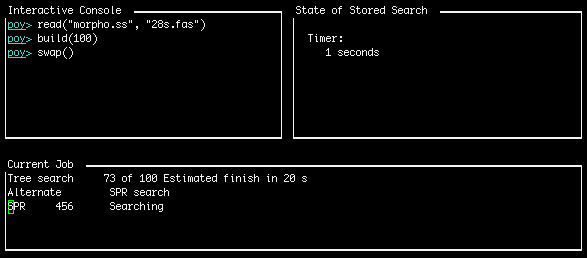
\includegraphics[width=\textwidth]{doc/figures/swap1.jpg}
\end{minipage}
\quad
\begin{minipage}[c]{0.453\textwidth}
	   	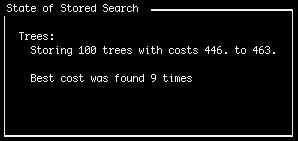
\includegraphics[width=\textwidth]{doc/figures/swap2.jpg}
   	\end{minipage}
\caption{Performing a local search. When searching (left panel), the \emph{Current Job} window reports the number of the tree that is currently being analyzed (\texttt{73 of 100}), a method of branch swapping (\texttt{Alternate}), a function being currently performed (\texttt{SPR search}), and a cost of the current tree (\texttt{456}). When the searching is finished (right panel), the \emph{State of Stored Search} window displays the best (\texttt{446}) and worst (\texttt{463}) costs, the number of trees stored in memory (\texttt{100}), and the number of trees of the best cost cost (\texttt{9}) recovered from independent tree builds. Note these trees may not necessarily have unique topologies.} 
\label{fig:swapping}
\end{figure}

Using different combinations of \commandstyle{swap()} arguments allows designing a  large number of search strategies of different levels of complexity. Some simple options allow the choice between SPR and TBR. More complex strategies allow keeping a specific number of best trees per single initial tree (generated during the building step). For example, the command \commandstyle{swap(trees:10)} will keep up to 10 best trees generated during branch swapping on a single initial tree. Consequently, if 100 trees were built initially, this command will produce up to 1,000 trees. The argument \commandstyle{threshold} allows the retention of suboptimal trees within a specified percent of cost difference from the current best tree. For example, \commandstyle{swap(trees:20, threshold:10)} will execute a swap considering trees within a ten percent cost difference of the current best tree and retain the 20 minimal length swapped trees for each initial build. Other options provide the means to sample trees as they are evaluated, timeout after certain number of seconds, transform the cost regime, and other functions in conjunction with many \poy commands.

\subsection{Selecting trees}

Having performed the basic steps of importing character data, building initial trees, and conducting a simple local search, we obtained a set of local-optima trees in memory. Most of the time, a user would like to select only those trees that are both ptimal \emph{and} topologically unique. The default setting of the \commandstyle{select()} does exactly that. Adding \commandstyle{select()} to our example of command sequence for the basic analysis 
\begin{quote}
 	\commandstyle{read("morpho.ss","28s.fas")}\\
 	\commandstyle{build(100)}\\
	\commandstyle{swap()}\\
	\commandstyle{select()}
\end{quote}
selects only unique trees of best cost. The remaining trees are deleted from memory. The \emph{State of Stored Search} window reports the number and the cost of the best tree(s) (Figure~\ref{fig:select}).

\begin{figure}[]
    \begin{center}
        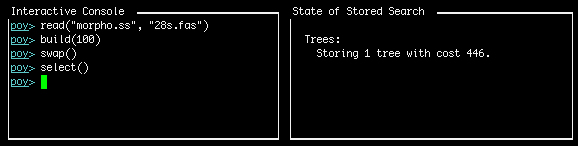
\includegraphics[width=0.6\textwidth]{doc/figures/select.jpg}
    \end{center}
    \caption{Selecting unique best trees. Executing \commandstyle{select()} keeps only unique trees of best cost. The \emph{State of Stored Search} window reports that there is only one unique tree of best cost (\texttt{446}).}
    \label{fig:select}
\end{figure}

This command \commandstyle{select()}, is another multifunctional command the arguments of which are also used to select (include or exclude) specific terminals, characters, and trees.) Comparing the output reported in the \emph{State of Stored Search} before (Figure~\ref{fig:swapping}) and after (Figure~\ref{fig:select}) executing \commandstyle{select()} shows that swapping on 9 of 100 initial trees produced the trees of best cost (\texttt{446}), but these trees are identical, because only one was retained when filtered using \commandstyle{select()}.

\subsection{Visualizing the results}

There are several options for visualizing results in \poy (see Section \ref{report}). The command
\commandstyle{report("my\_first\_tree", graphtrees)} outputs a cladogram in PDF format (Figure~\ref{fig:trees}), which can be displayed, edited, and printed using graphics software (such as Adobe Illustrator or Corel Draw). \poy also appends the ``ps'' extension when generating graphic output to a file. A quick way to see the tree(s) on screen is to use the command \commandstyle{report(asciitrees)} that draws a cladogram in the \emph{POY Output} window (Figure~\ref{fig:trees}). The ascii tree(s) can also be reported to a file, if an output file name is specified within the command (\commandstyle{report("my\_first\_trees", asciitrees)}).  These trees will be saved to a text file.

The command \commandstyle{report("my\_first\_trees.txt", trees)} reports the trees in memory in parenthetical notation to the file \texttt{my\_first\_trees} that can be imported in other programs. Other supported tree output formats include Newick and Hennig86. \commandstyle{report()} can also generate consensus trees in the graphical and parenthetical formats when appropriate arguments are specified (for example, \commandstyle{report("strict\_consensus", graphconsensus)}).

\begin{figure}
\centering
\begin{minipage}[c]{0.45\textwidth}
   		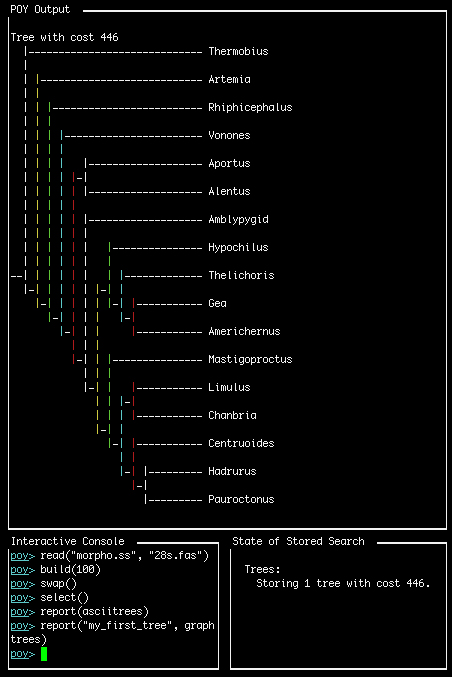
\includegraphics[width=\textwidth]{doc/figures/asciitree.jpg}
\end{minipage}
\quad
\begin{minipage}[c]{0.5\textwidth}
	   	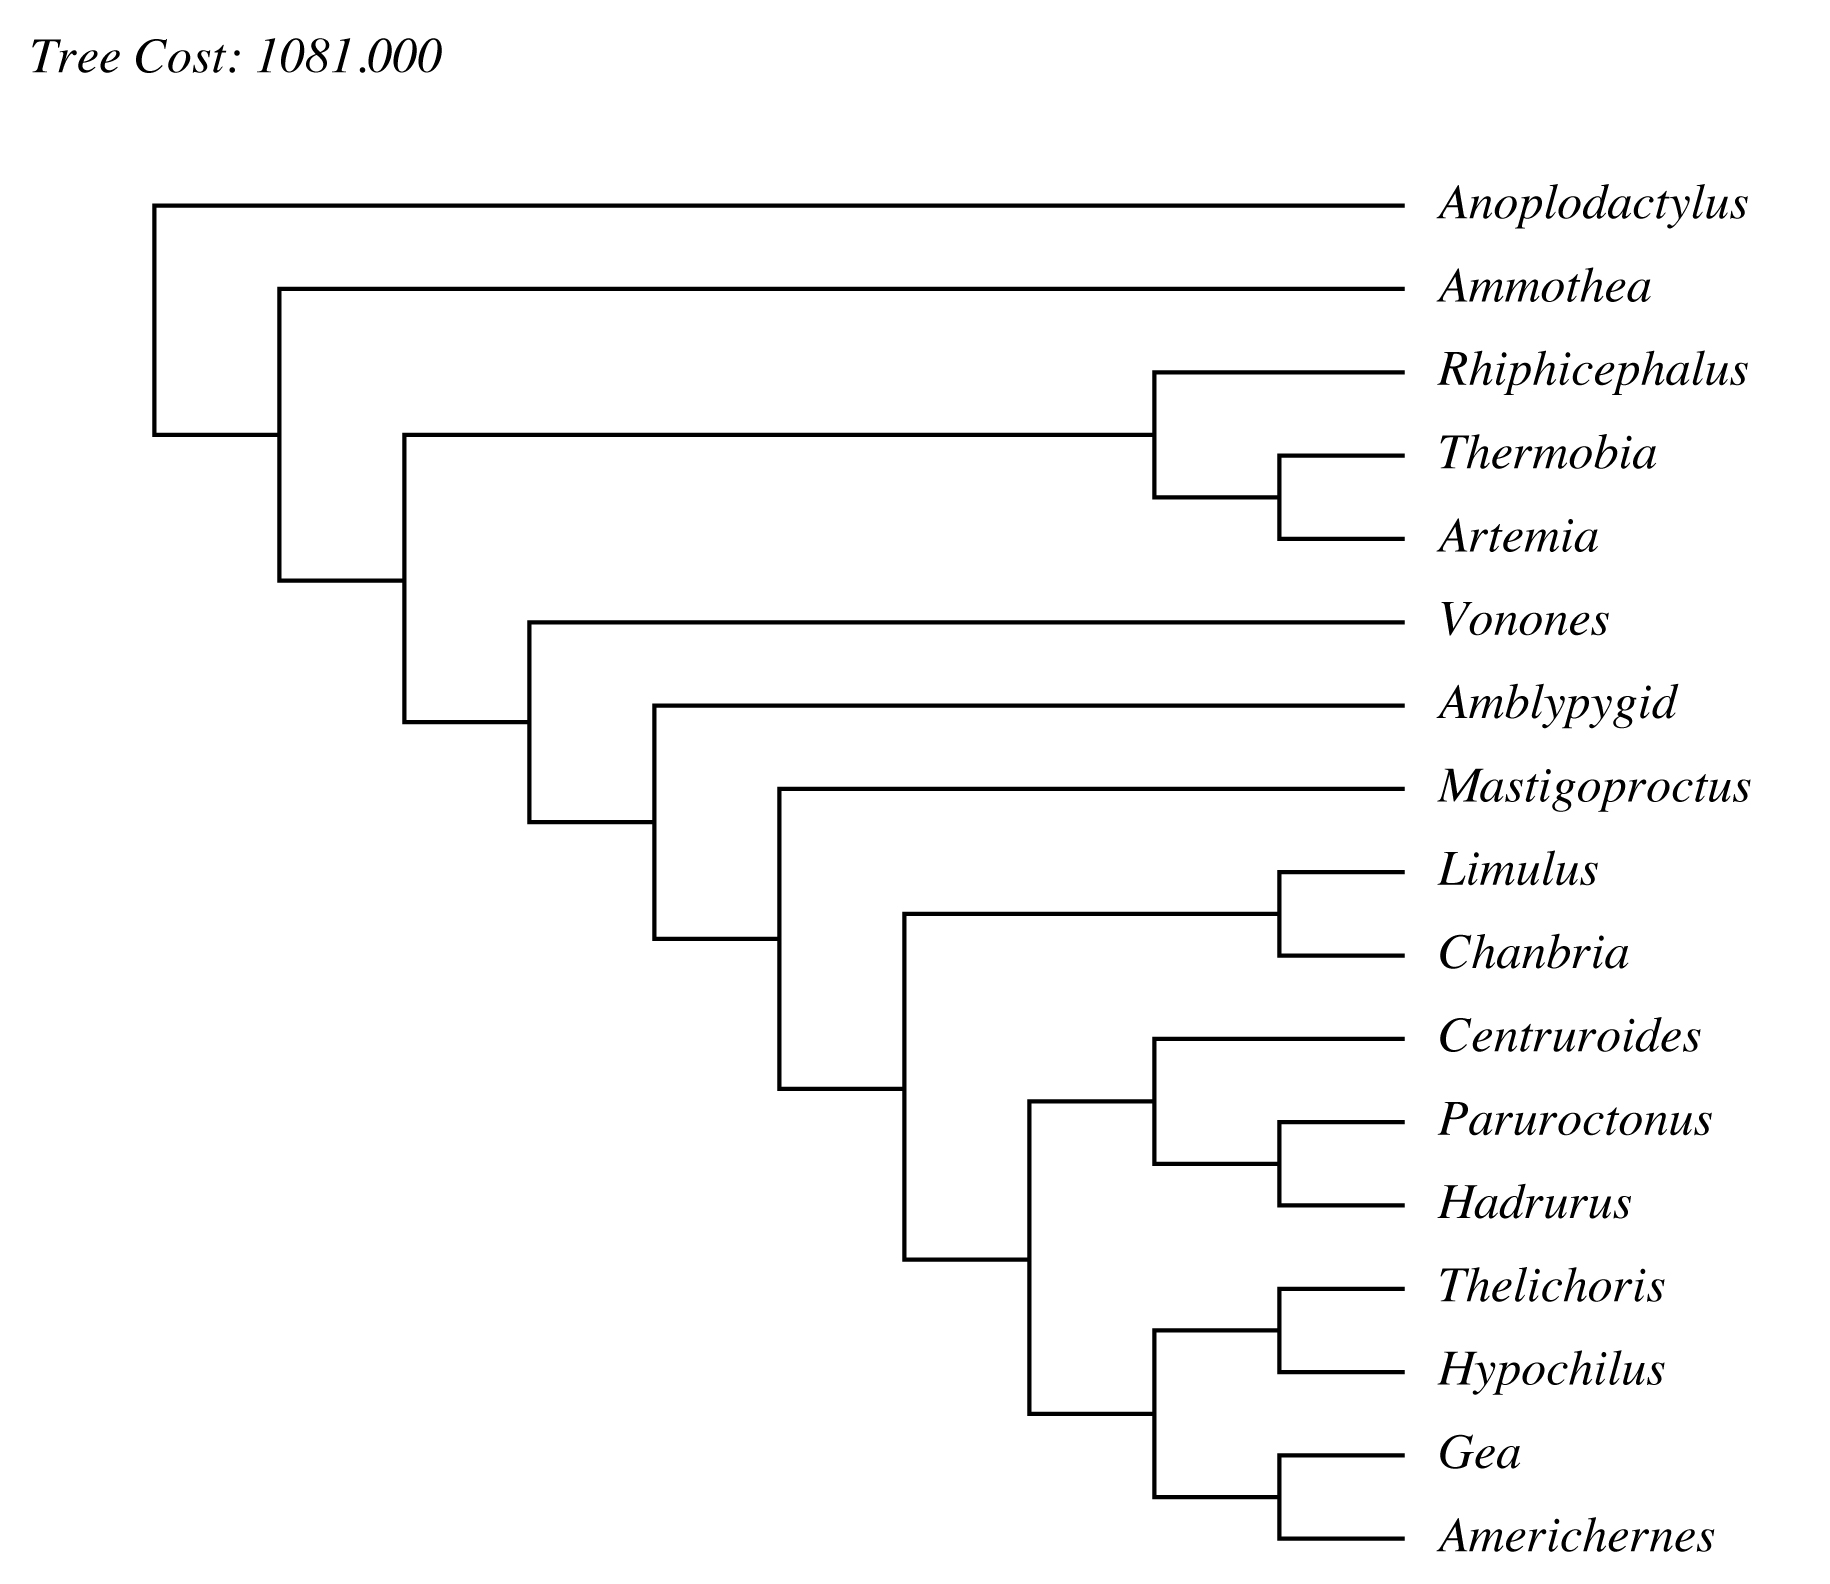
\includegraphics[width=\textwidth]{doc/figures/pstree.jpg}
   	\end{minipage}
\caption{Visualizing trees. An ascii tree (left) is generated using the command
\poycommand{report(asciitrees)}. The same tree is reported to a file in a PDF format (right) using \commandstyle{report("my\_first\_tree", graphtrees)}. Note that both representations of trees  are preceded by their costs.}
\label{fig:trees}
\end{figure}

\subsection{Interrupting a process}
To interrupt a process, press Control-C. By default, an error, \texttt{Error:}\\ \texttt{Interrupted}, is reported in the \emph{POY Output} window. The program does not close, however, and a new command can be entered. Interrupting the analysis cancels the execution of the last command requested by the user and restores the data and trees in memory before that last command. For example, the following two session are equivalent: 

\begin{quote}
 	\commandstyle{read("morpho.ss") <ENTER>} \\
\end{quote}
and

\begin{quote}
 	\commandstyle{read("morpho.ss") <ENTER>} \\
	\commandstyle{read("28s.fas", "18s.fas") <CONTROL-C>} \\
\end{quote}

In both of these sessions, only the morphological dataset ``morpho.ss'' is read into \poy.

\subsection{Reporting errors}
If there is an error pertaining to wrong syntax (such as a typo in a command name), \poy will indicate the location of the error by underlining the problematic part of the input with ``\texttt{\^}'' in the \emph{Interactive Console} (Figure~\ref{fig:errors}). The description of the corresponding command, its syntax, and examples of its usage from the help file are automatically printed in the \emph{POY Output} window. As noted above, the Up and Down keys can be used to scroll through the output and determine the source of the error. Certain types of errors are reported explicitly (Figure~\ref{fig:errors}).

\begin{figure}
\centering
\begin{minipage}[c]{0.48\textwidth}
   		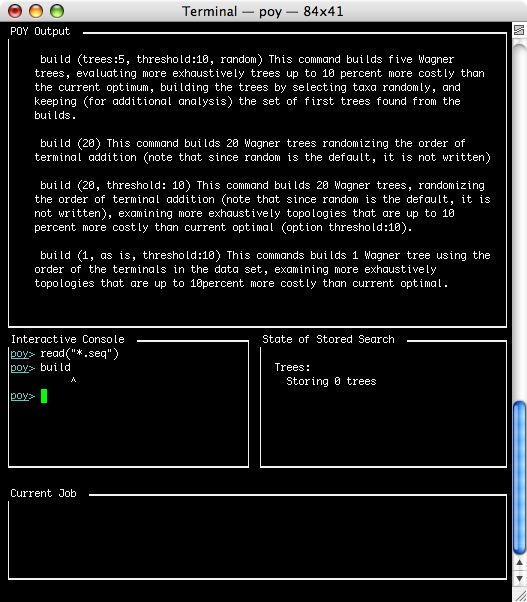
\includegraphics[width=\textwidth]{doc/figures/figerror1.jpg}
\end{minipage}%
\quad
\begin{minipage}[c]{0.48\textwidth}
	   	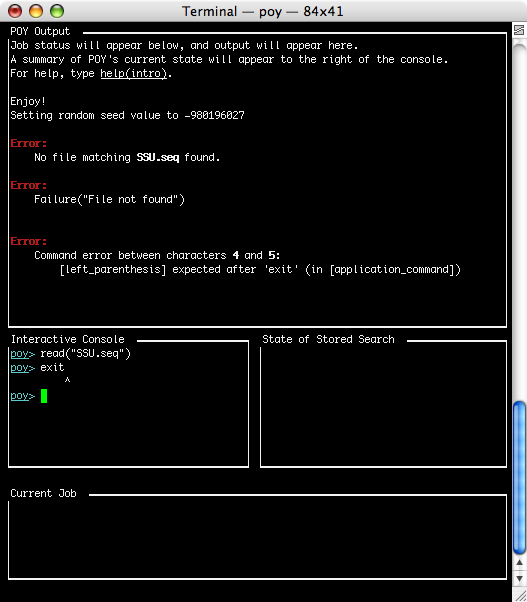
\includegraphics[width=\textwidth]{doc/figures/figerror2.jpg}
   	\end{minipage}
	
\caption{Displaying errors. \poy displays error messages in several ways. In the example in the left panel, the command \commandstyle{build} was entered without parentheses, which is required for a  valid \poy command syntax; the exact place of the error is marked by ``\texttt{\^}'', in this case  following the \commandstyle{build} commands. Examples of the proper usage of the command are automatically displayed in the \emph{POY Output}. In other cases (right panel), error messages are explicitly reported in the \emph{POY Output} window. The first and second error messages indicate that the data file \texttt{SSU.seq} is not present, which could have been caused either by a mistake in the name of the file, missing file, or the location of the file in a directory, other than the one specified prior to starting the \poy session. The third error message indicates that the valid syntax of \commandstyle{exit} requires the parentheses following the command name (also shown by ``\texttt{\^}'' in  the \emph{Interactive Console}).}
\label{fig:errors}
\end{figure}

\subsection{Exiting}
To finish a \poy session, enter the command \commandstyle{exit()} (Figure~\ref{fig:exithelp}) or \commandstyle{quit()}. This will close the \poy interface and resume the Terminal window (Mac OSX) or the Command Prompt window (Windows).

\begin{figure}[]
    \begin{center}
        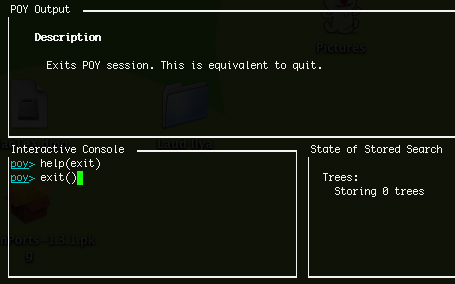
\includegraphics[width=0.5\textwidth]{doc/figures/exithelp.jpg}
    \end{center}
    \caption{Exiting \poy}
    \label{fig:exithelp}
\end{figure}

\section{Creating and running \poy scripts}

So far, we have communicated with \poy interactively through the \emph{Graphical User Interface} or by executing commands from the \emph{Interactive Console}. Another way of conducting an analysis is to run a \emph{script}, a simple text file containing a list of commands to be performed (Figure~\ref{fig:script}). 

Running analyses using scripts has many advantages: not only does it allow for the entire analysis to proceed from the beginning to the end at one click of a button, but it also provides means to examine the logical dependency of the commands and optimize memory consumption (see the description of \poyargument{script\_analysis} argument of the command \poycommand{report} in the \emph{POY Commands} chapter). Submitting jobs using scripts may produce results faster because \poy automatically optimizes the workflow of the entire analysis by taking into account the functional relationships among various tasks and efficiently distributing the jobs and resources (such as memory and multiple processors).

Another advantage of using scripts is that they may contain comments that are ignored by \poy but can be helpful to describe the contents of the files and provide other annotations. The comments are enclosed in parenthesis \emph{and} asterisks. For example, \texttt{(* this is a comment *)}. Comments can be of any length and span multiple lines. Comments can also be entered interactively from the \emph{Interactive Console}.

Obviously, using scripts requires the user to design the workflow of the process prior to conducting the analysis. \poy scripts can be created and saved using the \emph{Script Editor} window of the \poy \emph{Graphical User Interface} or any conventional text editor (such as TextPad, TextWrangler, BBEdit, Emacs, or NotePad).

\poy scripts are extremely useful in cases when operations may take a long time to complete, eliminating the need to wait for a part of the analysis to finish in order to proceed to the next step.

There are two ways to import and run a script:
\begin{itemize}
    \item using the \emph{POY Launcher} in the \emph{Graphical User Interface};
    \item using the command \commandstyle{run()} of the \emph{Interactive Console}; for example, \texttt{run("script.txt")}, where \texttt{script.txt} is the name of the file containing the script.
\end{itemize}

It it critical to include the command \commandstyle{exit()} at the end of the script. Otherwise \poy will be waiting for further instructions to be entered after executing the script's contents.

\begin{figure}
\centering
\begin{minipage}[c]{0.42\textwidth}
   		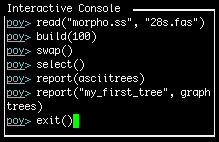
\includegraphics[width=\textwidth]{doc/figures/commandlist.jpg}
\end{minipage}
\,
\begin{minipage}[c]{0.53\textwidth}
	   	\includegraphics[width=\textwidth]{doc/figures/script.jpg}
   	\end{minipage}
\caption{Using \poy scripts. The list of commands executed interactively using the \emph{Interactive Console} (left) and a script containing the same list of commands (right). Note, that the header of the script is a comment, enclosed in ``(* *)'', that is ignored by \poy. Also note, that commands can either be listed in a row or in a column (compare \commandstyle{build()} and \commandstyle{swap()} in the console and in the script) and different arguments of the same command can either be specified separately or combined in a single argument list (compare \commandstyle{report()} in the console and in the script). (Both conventions are valid for interactive command submission and for scripts.)}
\label{fig:script}
\end{figure}

\section{Obtaining help} \label{sec:help}
Instructions to run \poy, command descriptions, and the theory behind \poy can be obtained from a variety of sources.
\begin{description}
\item[POY5.0 Program Documentation] (this manual) is a comprehensive and detailed manual on all the aspects of using \poy, from installation to output and visualization of results. Included are \emph{Quick Start}, \poy command reference, practical guides and tutorials that make the program immediately accessible for beginners and provide in-depth information for experienced users. The documentation in PDF format can be accessed from the \emph{Help} menu of the graphical user interface or downloaded separately from \poy web site at
\begin{center}
\texttt{http://research.amnh.org/scicomp/projects/poy.php}
\end{center}
\item[POY] interactive help can be obtained by entering \commandstyle{help()} at the \poy interactive console. To obtain help on a particular command, the name of the command must be specified in the parentheses following \commandstyle{help()}. For example, to learn about the command \commandstyle{exit}, type \commandstyle{help(exit)}. (Figure~\ref{fig:exithelp}.)
\item[POY5 Mail Group] is an Internet-based forum for discussing all issues related to \poy and provides the best way to communicate with \poy developers on specific issues (see \emph{WWW resources} below). The website is located at \texttt{http://groups.google.com/group/poy5}. \hl{new link}
\item[POY Book] (Wheeler et al., 2006 \emph{Dynamic Homology and Phylogenetic Systematics: A Unified Approach Using POY \cite{wheeleretal2006}}) provides a review of the theory behind \texttt{POY4} and by extension \poy, and contains formal descriptions of many algorithms implemented in the program and the descriptions of commands of the earlier version, \texttt{POY3}.
\begin{figure}[htbp]
   \centering
   \includegraphics[width=0.23\textwidth]{doc/figures/figpoybook.jpg}
   \caption{The POY Book.}
   \label{fig:figprocess}
\end{figure}
\end{description}

\section{WWW resources}
\poy is an ongoing project and new versions are being continuously developed to include new procedures, improve performance, and eliminate reported bugs. Therefore, it is imperative to keep up with the program's development and check regularly for updates. There are several Internet-based resources that offer this information.

\begin{description}
\item[POY5 Web Site] has downloadable compressed files of \poy binaries, source code, and documentation in PDF format. It also provides a links to the \emph{POY Mail Group}. The website is hosted by AMNH Computational Sciences at 
\begin{center}
\texttt{http://research.amnh.org/scicomp/projects/poy.php}
\end{center}

\item[POY5 source code repository] contains has downloadable \poy source code.  The site is powered by Google at 
\begin{center}
\texttt{http://code.google.com/p/poy5/source} \hl{new link}
\end{center}

\item[POY5 Mail Group] informs registered users via email of new developments, such as new versions and updates. It also provides  additional resources for obtaining help and a way for reporting bugs and other problems with \poy and its documentation. In addition, it allows users to receive and respond to each other's questions thus providing an open forum to  discuss the methods and applications of \poy. The users who choose not to register, have access to the archives of the postings but will not be able to either submit or receive emails from other users and \poy developers. The \emph{POY5 Mail Group} is hosted  by Google at
	\begin{center}
	\texttt{http://groups.google.com/group/poy5}  \hl{new link}
	\end{center}
	
\end{description}

%\begin{figure}[htbp]
%  \centering
%  \includegraphics[width=0.7\textwidth]{doc/figures/figprelim1.jpg}
%  \caption{Specifying the location of data files. The folder \texttt{POY-Data} is dragged from the \texttt{POY v3-4} folder directly in the Terminal window.}
%   \label{fig:figprelim1}
%\end{figure}%

%\begin{figure}[htbp]
%   \centering
%   \includegraphics[width=0.7\textwidth]{doc/figures/figprelim2.jpg}
%   \caption{Starting \poy. At the folder containing data files, entering \texttt{poy} starts a \poy session.}
%   \label{fig:figprelim2}
%\end{figure}%
